
\section{Proverif}
Let us start with a brief overview of Proverif internal reasoning. For more information, please refer to \cite{SymbolicComputationalBlanchet, SymbolicVerificationBlanchet, ProverifManual}.

\subsection{High level view}
Proverif protocols and security properties are based on an extended version of the \pic (the \textit{applied} \pic). The tool also allows the user to define constructors, destructors and equations\footnote{Destructors are basically used to de-construct some previously constructed term (e.g. decryption of an encrypted ciphertext), while equations represent term equality of some sort (e.g. commutativity of multiplication).}, which form the cryptographic primitives. The protocol is then automatically translated to a set of Horn-clauses. Using this abstract representation of the protocol (based on Horn-clauses), the Proverif verifier uses a resolution algorithm on such clauses that allows for verification of security properties \cite{SymbolicComputationalBlanchet}.
A graphical representation of the whole process is given in \cref{fig:proverif-verification-method}.

It is important to note that Proverif is not complete. This means that it may find false attacks. Moreover, it may not terminate, but it has been proven to be precise and efficient enough in practice by many case studies (the following is a non-exhaustive list of examples \cite{10.1145/1266977.1266978, ABADI20053, hal-01575923, DBLP:journals/corr/abs-2012-03141}).

We will now proceed with an overview of \pic and Horn-clauses.

\begin{figure}[t]
    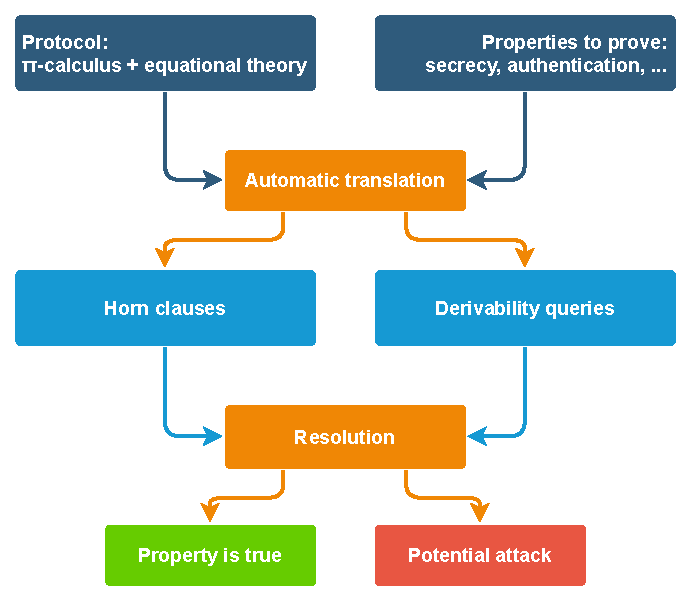
\includegraphics{proverif-verification-method}
    \centering
    \caption{Proverif verification method.\\Inspired by a representation from Bruno Blanchet \cite{SymbolicComputationalBlanchet}.}
    \label{fig:proverif-verification-method}
\end{figure}

\subsection{\pic and applied \pic}

The \pic \cite{pi-calculus-book} is a (minimal) programming that models system communicating on channels. It belongs to the \textit{process calculi} family, which is generally used to model concurrent systems. As Proverif uses the \textit{applied} \pic (which is an extension of standard \picnospace), we are going to briefly present its syntax in the rest of this section.

The following description of applied \pic references articles \cite{applied-pi-calculus-private-auth, applied-pi-calculus-abadi-1, applied-pi-calculus-abadi-2}. Please refer to these resources for further information and a more formal or in-depth description. For brevity, we only define main features of applied \pic in \cref{subsub:syntax-apic}.

\subsubsection{Overview of the syntax of the applied \pic}
\label{subsub:syntax-apic}

A \textit{signature \textSigma} is composed by a finite number of functions symbols, each with its own integer arity. Given such signature, together with an infinite set of names and an infinite set of variables, the set of \textbf{terms} is defined by the grammar:

\begin{equation}
\label{eq:apic-terms}
\begin{aligned}
    U, V &::=\\
    &a, b, \dots\\
    &x, y, \dots\\
    &f\left(U_1, \dots, U_l\right)
\end{aligned}
\qquad
\begin{aligned}
    \mbox{term}&\mbox{s}\\
    &\mbox{name}\\
    &\mbox{variable}\\
    &\mbox{constructor application}
\end{aligned}
\end{equation}

where $f \in \Sigma$ and $l$ matches the arity of $f$. Next, we define a grammar for processes, which is shown in \cref{eq:apic-processes}. As pointed to by Microsoft researchers, this grammar is very similar to the \pic \cite{applied-pi-calculus-private-auth}. We will omit defining differences from standard \pic as we have not formally defined \pic either.

\begin{equation}
\label{eq:apic-processes}
\begin{aligned}
    P, Q &::= \\
    &0 \\
    &\apicout{N}{M}{P} \\
    &\apicin{N}{x}{T}{P} \\
    &\apicpc{P}{Q}\\
    &\apicrep{P}\\
    &\apicnew{a}{T}{P}\\
    &\apicif{M}{P}{Q}
\end{aligned}
\qquad
\begin{aligned}
    \mbox{proc}&\mbox{esses} \\
    &\mbox{null process}\\
    &\mbox{output to channel N of message M}\\
    &\mbox{input from channel N of message M with sort T}\\
    &\mbox{parallel composition}\\
    &\mbox{replication}\\
    &\mbox{fresh value of sort T}\\
    &\mbox{conditional}
\end{aligned}
\end{equation}

The null process $0$ does nothing;
$\apicout{N}{M}{P}$ ($\apicin{N}{x}{T}{P}$) outputs (gets) the message M (of sort $x$) into (from) channel N and then continues with process $P$; Notice that getting a message from a channel is a blocking operation;
$\apicpc{P}{Q}$ is the parallel composition of $P$ and $Q$;
The process $\apicrep{P}$ effectively behaves as an infinite number of copies of $P$ running in parallel (\textit{unbounded} replication);
$\apicnew{a}{T}{P}$ creates a new fresh value of sort $T$, before proceeding with process $P$;
$\apicif{M}{P}{Q}$ if a standard conditional.

\comment{
$\apiclet{x}{T}{D}{P}{Q}$ is used to apply destructors or assign some term $D$ to a variable $x$ (of sort $T$);
} 



\subsection{Horn-clauses}







\section{Tamarin-prover}
In this section we will see an overview of Tamarin foundations and internal reasoning.
For a more in-depth description and further information, see the Tamarin foundations paper \cite{TamarinFoundations} or the extended foundations paper \cite{TamarinFoundationsExtended}.

\subsection{High level view}
First of all, let us examine an high level picture of Tamarin.

The security property model of Tamarin is based on labelled multiset rewriting rules to specify protocols and adversary capabilities, a guarded fragment\footnote{Only a few examples of formulas respecting the guarded fragment of first order logic used by Tamarin will be given in \cref{sub:guarded-formulas}. See \cite{FragmentFirstOrderLogicPaper} for a rigorous definition from a mathematical point of view.} of first order logic to specify security properties\footnote{Security properties in Tamarin will also be referred to as \textit{lemmas}.} and functions and equational theories to model the algebraic properties of cryptographic protocols \cite{TamarinFoundations}.

Given the rewriting rules, security properties and equational theories, Tamarin uses a novel constraint-solving algorithm which tries to validate or falsify lemmas.

In other words, Tamarin allows to specify a labelled transition system that induces a set of traces and offers verification of such traces using a guarded fragment of first-order logic to specify ``good" traces. Tamarin then tries to prove the negation of the specified ``good" traces.

Tamarin also offers builtin equational theories \cite{TamarinProverManual}. A brief overview will be given in \cref{sub:Builtin-equational-theories}.

\subsection{Terminology}
As reported earlier, multiset rewriting rules are used to specify adversary capabilities and protocols. More precisely, a \textit{set} of \textit{labelled} multiset rewriting rules are used.

The ingredients of this multiset rewriting system are the following: 

\begin{description}[style=nextline]
    \item[Terms] which can be essentially thought of as messages. Terms can be of three different sorts. The more general sort is the \textit{msg} sort, which has two incomparable subsorts \textit{fresh} and \textit{pub} for fresh and public names, respectively;
    \item[Facts] which model information in the protocol. Facts have an arity, can be linear or persistent and are composed by terms. Linear facts model resources that can be consumed once, while persistent facts can be consumed an arbitrary number of times (and are prefixed by an exclamation mark). By convention, facts always start with a capital letter;
    \item[Special facts] Four facts are reserved and are used to model the freshness of a message $t$ ($\mbox{\textbf{Fr}}\left(t\right)$), a message $t$ coming from the public channel ($\mbox{\textbf{In}}\left(t\right)$), a message $t$ to be output to the public channel ($\mbox{\textbf{Out}}\left(t\right)$) and knowledge of a certain message $t$ from the attacker ($\mbox{\textbf{K}}\left(t\right)$);
    \item[State of the system] The state of the system is represented using a \textit{multiset} of facts;
    \item[Transition rules] A multiset of transition rules defines the possible transitions from one state to another one. Transitions are denoted with the following syntax
    \begin{equation}
        L \msrewrite{A} R
    \end{equation}
    where $L, A$ and $R$ are multisets of facts, respectively called \textbf{premises}, \textbf{actions} and \textbf{conclusions}.
    \item[Trace] A trace is a sequence $\left<A_1, \dots, A_n\right>$ of sets of ground facts denoting the sequence of actions that happened during a protocol's execution.
\end{description}


\subsection{Transition rules}
\label{sub:Transition-rules}
Let us examine an informal description of transitions.

\begin{itemize}
    \item{Let $S$ be the current state of the system}
    \item{Let $\msrnolabel{L}{R}$ be a transition rule. Note that this is a \textit{multiset rewriting rule} without a \textit{label};}
    \item{Let $\msrnolabel{l}{r}$ be a ground instance of the rule (i.e. no variables are present in the multisets);}
    \item{If we apply $\msrnolabel{l}{r}$ (assuming $l \msrsubseteq S$) to our state $S$ we reach a new state, defined by the following equation:
    \begin{equation}
        S' = S \msrsetminus l \msrcup r
    \end{equation}
    We use $\msrsetminus$, $\msrcup$ and $\msrsubseteq$ to define difference, union and subset over multisets, respectively. We can also consider the difference between linear and persistent facts and define $\lin{l}$ ($\pers{l}$) as linear facts (persistent facts) in $l$. Assuming that $\lin{l} \msrsubseteq S$ and $\pers{l} \msrsubseteq S$, then the equation becomes the following:
    \begin{equation}
        S' = S \msrsetminus \lin{l} \msrcup r
    \end{equation}
    It should be fairly clear from the equation why persistent facts can be consumed any number of times: they are never removed from the state of the system. This can be useful in scenarios in which we want to model persistent knowledge (e.g. the establishment of an encryption key $k$ may be expressed by a persistent fact $\fact{Key}{k}$).
    }
    \item{When we use labelled multiset rewriting rules, such as $\msr{l}{a}{r}$, we also add facts from $a$ to the \textit{trace} of the execution.}
\end{itemize}

\Cref{eq:builtin-tamarin-msr-rules} shows multiset rewriting rules that are always defined by Tamarin. It is not hard to see that these equations are used to model the Dolev-Yao attacker: the first rule allows the adversary to send a message $x$ he knows to someone, while the second one allows him to learn a message $x$ sent by someone.

\begin{equation}
\label{eq:builtin-tamarin-msr-rules}
\begin{gathered}
    \msr{!KU\left(x\right)}{K\left(x\right)}{In\left(x\right)}\\
    \msrnolabel{Out\left(x\right)}{\ !KD(x)}
\end{gathered}
\end{equation}


\subsection{Builtin equational theories}
\label{sub:Builtin-equational-theories}
A brief list of Tamarin built-ins is given below. Only the builtin theories considered relevant and those used in the analysis will be described here. The full list is available in the Tamarin manual. \cite{TamarinProverManual}.

\begin{description}[style=nextline]
    \item[hashing] defines a perfect hash function \textbf{h/1}\footnote{The writing \textbf{f/x} indicates that the function \textbf{f} has arity \textbf{x}.};
    \item[asymmetric-encryption] models a public key encryption scheme. It defines the following symbols:
    
    \begin{itemize}
        \item{\textbf{aenc/2}, used to model the encryption of a message with a public key}
        \item{\textbf{adec/2}, used to model the decryption of an encrypted message with a private key}
        \item{\textbf{pk/1}, used to derive a public key from a private key}
    \end{itemize}

    Functions are related by the equation \textbf{adec(aenc(msg, pk(sk)), sk) = msg};

    \item[diffie-hellman] models Diffie-Hellman groups. It defines the following symbols:
    
    \begin{itemize}
        \item{\textbf{inv/1}, models the inverse of an element}
        \item{\textbf{1/0}, models the neutral element}
        \item{\textbf{$\myexp$} and \textbf{*} symbols, models exponentiation and multiplication respectively}
    \end{itemize}

    The equational theory for this builtin is actually quite complex. For the sake of completeness, these are the related equations:
    \begin{equation}
    \begin{aligned}
        &x \myexp y \myexp z = x \myexp \left(y * z\right) \\
        &x ^ 1 = x \\
        &x * y = y * x \\
        &\left(x * y\right) * z = x * \left(y * z\right) \\
        &x * 1 = x \\
        &x * inv\left(x\right) = 1
    \end{aligned}
    \end{equation}
    % TODO: parla ancora un po' di quanto sia figo Tamarin che ha DH builtin!
\end{description}

\subsection{Guarded formulas}
\label{sub:guarded-formulas}

As reported earlier, Tamarin uses a guarded fragment of first order logic to specify security properties and $-$ in general $-$ traces. All formulas must be guarded, which essentially means that all variables quantified \textbf{must} appear in facts. \Cref{eq:guarded-formulas} shows two main formulas that respect the guarded fragment. Most $-$ if not every $-$ security property can be expressed using these formulas:

\begin{equation}
\label{eq:guarded-formulas}
\begin{gathered}
    \forall \overline{x}. F\left(\overline{z}\right) @i \Rightarrow \psi \\
    \exists \overline{x}. F\left(\overline{z}\right) @i \land \psi
\end{gathered}
\end{equation}

where $F$ is a fact, $\psi$ is guarded and $\overline{x}$ and $\overline{z}$ are vectors of terms such that $\overline{x} \subseteq \overline{z} \cup i$.
The variable $i$ is a timepoint, which annotates that the fact $F$ occurred at time $i$ (timepoints all belong to $\Q$)\footnote{Notice that timepoints are very useful to define post-compromise security properties (i.e. leaking an ephemeral key \textbf{after} honest parties have used it) and Perfect Forward Secrecy.} \cite{TamarinTeachingSlides}.

\section{Comparison of Proverif and Tamarin}
\label{section:proverif-vs-tamarin}

\comment{
    Proverif is NOT complete (see SymbolicComputationalBlanchet page 10), while Tamarin actually is (probably see foundations paper).
}